\documentclass[11pt,a4paper]{ctexart}

\usepackage[margin=2.6cm]{geometry}
\usepackage{amsmath,amssymb,amsthm}
\usepackage{graphicx}
\usepackage{booktabs}
\usepackage{hyperref}
\usepackage{xcolor}
\usepackage{listings}
\usepackage{caption}

\graphicspath{{figures/}}
\hypersetup{colorlinks=true, linkcolor=blue!50!black, urlcolor=blue!60!black}
\lstset{
  basicstyle=\ttfamily\small,
  breaklines=true,
  frame=single,
  columns=fullflexible,
  backgroundcolor=\color{gray!7}
}

\newtheorem{definition}{定义}[section]
\newtheorem{theorem}{定理}[section]
\newtheorem{lemma}{引理}[section]
\newtheorem{proposition}{命题}[section]
\newtheorem{example}{例}[section]

\title{第 4 章 \quad Linear time series / 线性时间序列}
\author{基于 \textit{A Course in Time Series Analysis} 的中文讲义与 Python 实践}
\date{}

\begin{document}
\maketitle

\section*{本章学习目标}

本章按照原文 \textit{Linear time series} 的小节顺序整理，保留主要定义、定理、模型公式和练习方向，并将原文中的 R 实践思路改写为 Python 工程实践。

完成本章后，应能够：
\begin{itemize}
  \item 理解线性过程和 \(MA(\infty)\) 表示；
  \item 掌握后移算子、AR(p) 差分方程和因果解；
  \item 说明 AR(2) 的伪周期现象和季节 AR 模型；
  \item 区分 AR、MA、ARMA 的因果性与可逆性；
  \item 理解单位根、非可逆过程以及 ACF/PACF 诊断。
\end{itemize}

\section{动机}

线性时间序列把当前观测表示为过去冲击的线性组合。它是全书的工作马模型：既能产生丰富的相关结构，又有清晰的协方差、预测和频域公式。

\section{线性过程与移动平均模型}

\begin{definition}[线性过程与 \(MA(\infty)\)，原文 Definition 4.2.1]
若 \(\{\varepsilon_t\}\) 是均值为 0、方差为 \(\sigma^2\) 的不相关创新，且
\[
  X_t=\sum_{j=0}^{\infty}\psi_j\varepsilon_{t-j},
  \qquad \sum_{j=0}^{\infty}|\psi_j|<\infty,
\]
则称 \(\{X_t\}\) 是线性过程，也称具有 \(MA(\infty)\) 表示。
\end{definition}

\begin{lemma}[无限和的存在性，原文 Lemma 4.2.1]
若系数满足适当可和条件且创新二阶矩有限，则上述无限和在均方意义下存在，并定义一个二阶平稳过程。
\end{lemma}

其均值为 0，自协方差为
\[
  c(k)=\sigma^2\sum_{j=0}^{\infty}\psi_j\psi_{j+|k|}.
\]

\section{AR(p) 模型}

\subsection{差分方程与后移算子}

后移算子定义为 \(BX_t=X_{t-1}\)。AR(p) 模型写作
\[
  X_t=\phi_1X_{t-1}+\cdots+\phi_pX_{t-p}+\varepsilon_t,
\]
或
\[
  \phi(B)X_t=\varepsilon_t,\qquad
  \phi(z)=1-\phi_1z-\cdots-\phi_pz^p.
\]

\subsection{AR(1) 的两个解}

对
\[
  X_t=\phi X_{t-1}+\varepsilon_t,
\]
若 \(|\phi|<1\)，因果平稳解为
\[
  X_t=\sum_{j=0}^{\infty}\phi^j\varepsilon_{t-j}.
\]
若 \(|\phi|>1\)，也可构造非因果平稳解
\[
  X_t=-\sum_{j=1}^{\infty}\phi^{-j}\varepsilon_{t+j},
\]
但该解依赖未来创新，不适合作为预测模型。

\begin{lemma}[AR(p) 因果解，原文 Lemma 4.3.1]
若 \(\phi(z)\) 的所有根都在单位圆外，则 AR(p) 有唯一因果平稳解，且可写成
\[
  X_t=\sum_{j=0}^{\infty}\psi_j\varepsilon_{t-j},
\]
其中 \(\psi(z)=1/\phi(z)\) 在单位圆附近解析。
\end{lemma}

\section{AR(2)、伪周期与季节自回归}

AR(2) 的特征根若为复数，会产生阻尼振荡。若根可表示为 \(re^{\pm i\omega}\)，则样本路径和自协方差常表现出近似周期
\[
  P=\frac{2\pi}{\omega}.
\]
这就是原文称为 pseudo periodicity 的现象：模型没有确定性周期项，但相关结构会产生类似周期的波动。

季节自回归模型把滞后设为季节长度，例如月度数据中常见
\[
  X_t=\Phi X_{t-12}+\varepsilon_t.
\]
它用于刻画每年同月之间的相关性。

\section{ARMA 模型}

\begin{definition}[AR、ARMA 与 MA，原文 Definition 4.5.1]
ARMA(p,q) 模型定义为
\[
  \phi(B)X_t=\theta(B)\varepsilon_t,
\]
其中
\[
  \phi(z)=1-\phi_1z-\cdots-\phi_pz^p,\qquad
  \theta(z)=1+\theta_1z+\cdots+\theta_qz^q.
\]
当 \(q=0\) 时为 AR(p)，当 \(p=0\) 时为 MA(q)。
\end{definition}

\begin{definition}[因果与可逆，原文 Definition 4.5.2]
若 \(\phi(z)\) 的根都在单位圆外，则模型因果；若 \(\theta(z)\) 的根都在单位圆外，则模型可逆。可逆性保证创新可由当前和过去观测恢复：
\[
  \varepsilon_t=\sum_{j=0}^{\infty}\pi_j X_{t-j}.
\]
\end{definition}

\section{ARFIMA、单位根与诊断}

ARFIMA 模型通过分数差分 \((1-B)^d\) 描述长记忆。单位根模型含有 \(\phi(1)=0\)，最典型例子是随机游走
\[
  X_t=X_{t-1}+\varepsilon_t.
\]
诊断上，MA(q) 的 ACF 通常 q 阶截尾，AR(p) 的 PACF 通常 p 阶截尾；单位根过程的 ACF 衰减很慢，差分后更接近平稳。

\section{原文小节覆盖补充}

\subsection{无限随机变量和}
原文在定义线性过程前先处理无限随机变量和的收敛问题。若 \(\sum_jE|a_j\varepsilon_{t-j}|^2<\infty\)，则部分和在均方意义下收敛；这保证 \(MA(\infty)\) 表示真正定义了随机变量。

\begin{example}[原文 Example 4.2.1]
若 \(\{X_t\}\) 严格平稳且方差有限，定义 \(Y_t=\sum_{j=0}^{\infty}a_jX_{t-j}\)，则在系数足够可和时，\(Y_t\) 也是良好定义的平稳线性滤波序列。
\end{example}

\subsection{两个 AR(1) 解和一般 AR(p) 解}
同一个 AR 方程可能有因果解和非因果解。因果解依赖过去创新，适合预测；非因果解依赖未来创新，通常只作为理论对照。Exercise 4.1 要求求 AR(1) 平稳解；Exercise 4.2 要求处理一般 AR(p) 表示。

\begin{lemma}[解析函数技术，原文 Lemma 4.3.2--4.3.3]
若 \(\phi(z)\) 在单位圆附近无零点，则 \(1/\phi(z)\) 可展开为收敛幂级数，因此 AR(p) 可写成 \(MA(\infty)\)。
\end{lemma}

\subsection{AR(2) 显式解、伪周期和周期图历史}
AR(2) 是展示阻尼振荡的最小模型。若特征根为复共轭，样本路径和 ACF 呈现伪周期。Exercise 4.3、Exercise 4.4、Exercise 4.5 和 Exercise 4.6 都围绕 AR(2) 因果条件、显式解和指定伪周期展开。

\begin{example}[伪周期 AR(2)]
当根为 \(re^{\pm i\omega}\) 时，自协方差含有 \(\cos(k\omega)\) 型项，周期近似为 \(2\pi/\omega\)。
\end{example}

\subsection{季节 AR、AR(\(\infty\)) 与模拟}
季节 AR 使用季节滞后，例如 \(X_t=\Phi X_{t-12}+\varepsilon_t\)。AR(\(\infty\)) 仍依赖系数可和和解析性。原文模拟部分强调，给定创新、初始值和递推公式即可生成 AR 样本；Exercise 4.7 要求用非高斯创新模拟。

\subsection{ARMA、ARFIMA、单位根、非可逆和诊断}
ARMA 综合 AR 的递推依赖与 MA 的冲击叠加；ARFIMA 用分数差分描述长记忆；单位根过程需要差分；非可逆 MA 虽可能有相同 ACF，但创新不能由过去观测稳定恢复。诊断部分强调 ACF/PACF 和单位根检查。

\subsection{4.8 模型模拟}
原文第 4.8 节把 AR、MA、ARMA、单位根模型的模拟统一为“生成创新后递推或滤波”。模拟用于理解样本路径、验证 ACF/PACF 诊断，也用于构造课堂实验。

\subsection{4.10 附录}
附录补充若干代数推导，帮助读者从特征根、多项式和递推公式之间来回转换。它不引入新模型，但支撑正文中 AR 解和 ARMA 表示的推导。

\section{Python 工程实践}

在本章目录下运行：
\begin{lstlisting}[language=bash]
python scripts/ch04_generate_figures.py
\end{lstlisting}

脚本会把图像写入本章 \texttt{figures/} 目录。当前图像用于配合本章核心概念的仿真说明；若后续补齐原始数据文件，可把模拟数据替换为原文真实数据案例。

\begin{figure}[htbp]
  \centering
  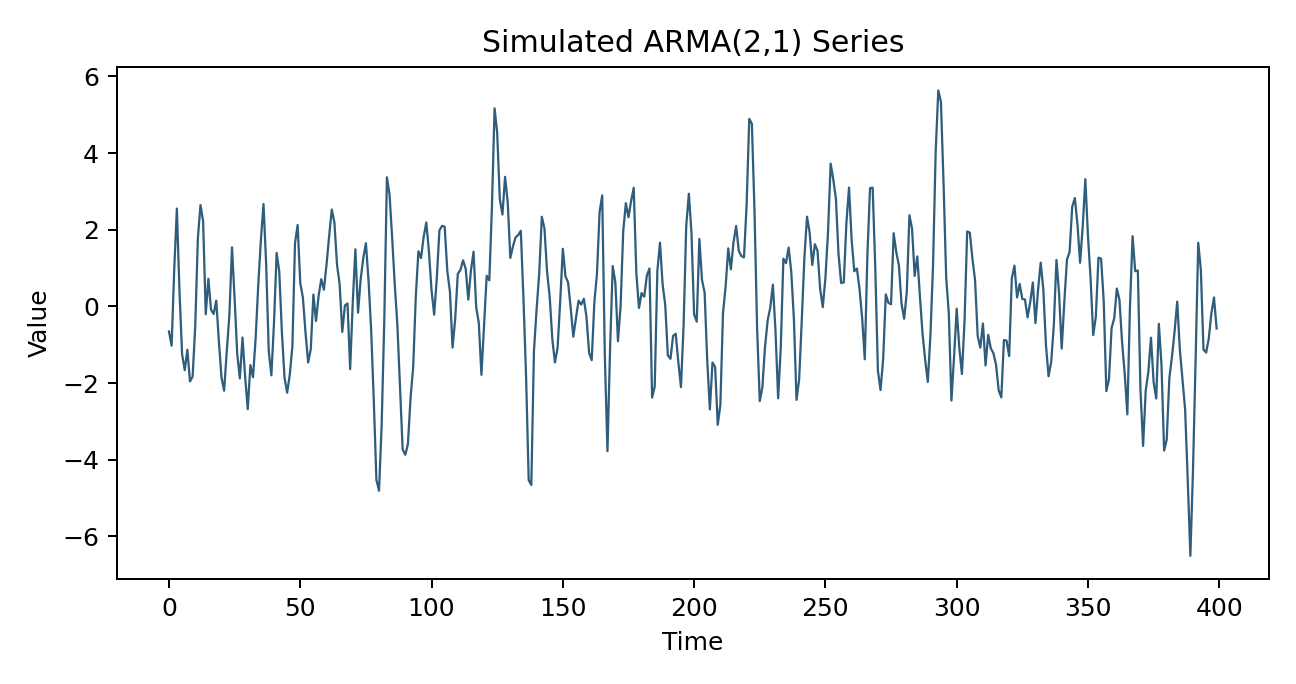
\includegraphics[width=0.86\textwidth]{ch04_fig01_arma_series.png}
  \caption{模拟 ARMA(2,1) 序列：线性模型可产生持续相关但均值稳定的波动。}
\end{figure}

\begin{figure}[htbp]
  \centering
  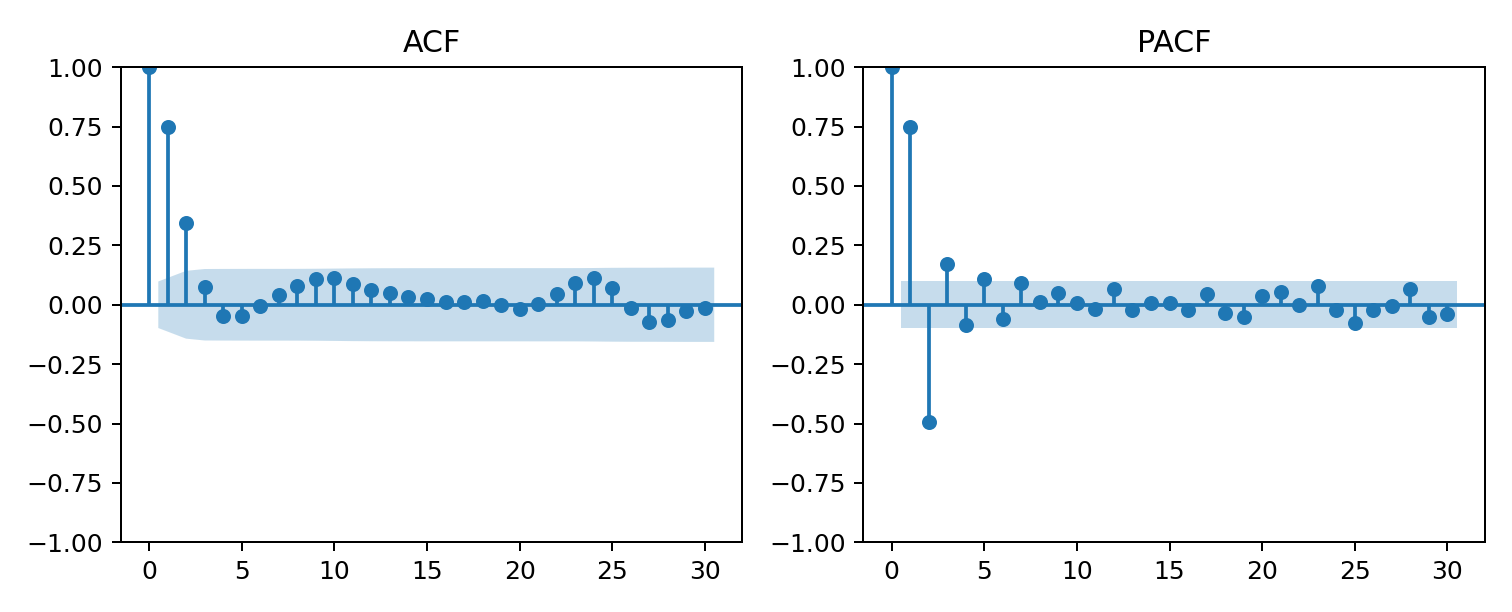
\includegraphics[width=0.86\textwidth]{ch04_fig02_acf_pacf.png}
  \caption{ACF/PACF 诊断图：用于区分 AR 与 MA 结构并辅助阶数选择。}
\end{figure}

\section{练习提要}

原文练习主要围绕下列方向展开：
\begin{itemize}
  \item 求 AR(1)、AR(2) 的平稳因果解；
  \item 根据特征根判断 AR(p) 的因果性；
  \item 构造具有指定伪周期的 AR(2) 模型；
  \item 模拟 ARMA、单位根和非可逆模型并比较 ACF/PACF。
\end{itemize}

\section*{本章小结}

第 4 章给出了线性时间序列的模型语言。后移算子把差分方程写成多项式，根的位置决定因果性、可逆性和单位根；ACF 与 PACF 则把这些理论结构变成可观察诊断。

\end{document}
